% !TEX encoding = UTF-8 Unicode
\documentclass[a4paper]{article}

\usepackage{color}
\usepackage[obeyspaces]{url}
\usepackage[T1]{fontenc} % enable Cyrillic fonts
\usepackage[utf8]{inputenc} % make weird characters work
\usepackage{graphicx}
\usepackage[margin=1.0in]{geometry}
\usepackage[table]{xcolor}
\usepackage{tocloft}
\usepackage{float}
\addtolength{\cftsecnumwidth}{10pt}
\usepackage{wasysym}


\usepackage[english,serbian]{babel}
%\usepackage[english,serbianc]{babel} 

\PassOptionsToPackage{obeyspaces}{url}
\usepackage[unicode]{hyperref}
\hypersetup{colorlinks,citecolor=green,filecolor=green,linkcolor=blue,urlcolor=blue}

\usepackage{listings}
\renewcommand\lstlistingname{Kod}
\renewcommand\lstlistlistingname{Kodovi}

\definecolor{mygreen}{rgb}{0,0.6,0}
\definecolor{mygray}{rgb}{0.5,0.5,0.5}
\definecolor{mymauve}{rgb}{0.58,0,0.82}

\lstset{
  backgroundcolor=\color{white},   % choose the background color; you must add \usepackage{color} or \usepackage{xcolor}; should come as last argument
  basicstyle=\scriptsize\ttfamily,        % the size of the fonts that are used for the code
  breakatwhitespace=false,         % sets if automatic breaks should only happen at whitespace
  breaklines=true,                 % sets automatic line breaking
  captionpos=b,                    % sets the caption-position to bottom
  commentstyle=\color{mygreen},    % comment style
  deletekeywords={...},            % if you want to delete keywords from the given language
  escapeinside={\%*}{*)},          % if you want to add LaTeX within your code
  extendedchars=true,              % lets you use non-ASCII characters; for 8-bits encodings only, does not work with UTF-8
  firstnumber=1,                   % start line enumeration with line 1000
  frame=single,	                   % adds a frame around the code
  keepspaces=true,                 % keeps spaces in text, useful for keeping indentation of code (possibly needs columns=flexible)
  keywordstyle=\color{blue},       % keyword style
  language=Python,                 % the language of the code
  morekeywords={*,...},            % if you want to add more keywords to the set
  numbers=left,                    % where to put the line-numbers; possible values are (none, left, right)
  numbersep=5pt,                   % how far the line-numbers are from the code
  numberstyle=\tiny\color{mygray}, % the style that is used for the line-numbers
  rulecolor=\color{black},         % if not set, the frame-color may be changed on line-breaks within not-black text (e.g. comments (green here))
  showspaces=false,                % show spaces everywhere adding particular underscores; it overrides 'showstringspaces'
  showstringspaces=false,          % underline spaces within strings only
  showtabs=false,                  % show tabs within strings adding particular underscores
  stepnumber=2,                    % the step between two line-numbers. If it's 1, each line will be numbered
  stringstyle=\color{mymauve},     % string literal style
  tabsize=2,	                     % sets default tabsize to 2 spaces
  title=\lstname                   % show the filename of files included with \lstinputlisting; also try caption instead of title
}

\usepackage{enumitem}
\newlist{legal}{enumerate}{10}
\setlist[legal]{label*=\arabic*.}

\begin{document}

\title{Informacioni sistem pozorišta\\ \small{Seminarski rad u okviru kursa\\Informacioni sistemi\\ Matematički fakultet}}

\author{
Katarina Savičić 1086/2020\\
Dragana Milić 1042/2019\\
Nikola Vuković 1090/2020\\
Ognjen Milinković 1008/2020\\
Momir Adžemović 1005/2020
}

\date{1.~april 2020.}

\maketitle

\abstract

Ovo je sažetak. On se piše na kraju.

\newpage

\tableofcontents

\newpage

\section{Uvod}
Ovaj rad se bavi modeliranjem najvažnijih procesa u radu jednog pozorišta, gde se akcenat
stavlja na proces produkcije predstave. Proces predstave se sastoji iz dva glavna 
dela\cite{hamilton_theatre_producing_the_drama}:
\begin{itemize}
  \item priprema i izvođenje
  \item tehnički deo
\end{itemize}

\section{Analiza sistema}
Informacioni sistem je namenjen korisnicima koji su zaposleni u pozorištu i klijentima, tj. posetiocima 
pozorišta. Izrađen je kao projekat u okviru predmeta "Informacioni sistemi" na master studijama Matematičkog fakulteta. 
Vođenje i organizacija rada pozorišta uključuje niz aktivnosti. U okviru ovog projekta urađene su 
sledeće funkcionalnosti:

  \begin{itemize}
    \item Organizacija predstave
    \item Rezervacija sala
    \item Održavanje repertoara
    \item Prodaja karata
    \item Vođenje finansija
  \end{itemize}
  
Na narednoj slici nalazi se dijagram toka podataka koji grafički prikazuje
osnovne aktere u sistemu i veze među njima.

\begin{figure}[H]
  \begin{center}
      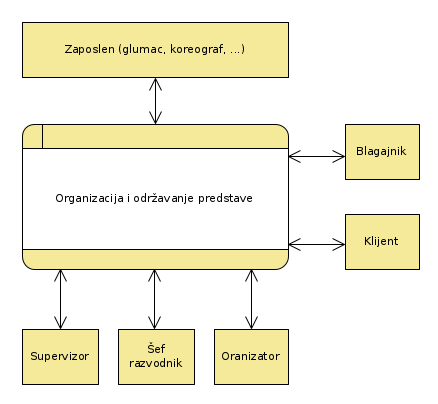
\includegraphics[width=80mm]{../images/dfd0.png}
  \end{center}
  \caption{Dijagram toka podataka nultog nivoa}
  \label{dfd0}
\end{figure}

Dijagram toka podataka prvog nivoa prikazuje detaljnije sistem. Iako su procesi "Registrovanje zaposlenih"
i "Registracija" (odnosi se na registrovanje klijenata) podslučajevi upotrebe, izdvojene su na narednom dijagramu,
jer se izdvajaju po interakciji između trećih lica i podataka od celovitog slučaja upotrebe. Za
procese sa identifikatorom 1, 3, 4, 5, i 6 se može videti u nastavku dijagram podataka drugog nivoa.

\begin{figure}[H]
  \begin{center}
      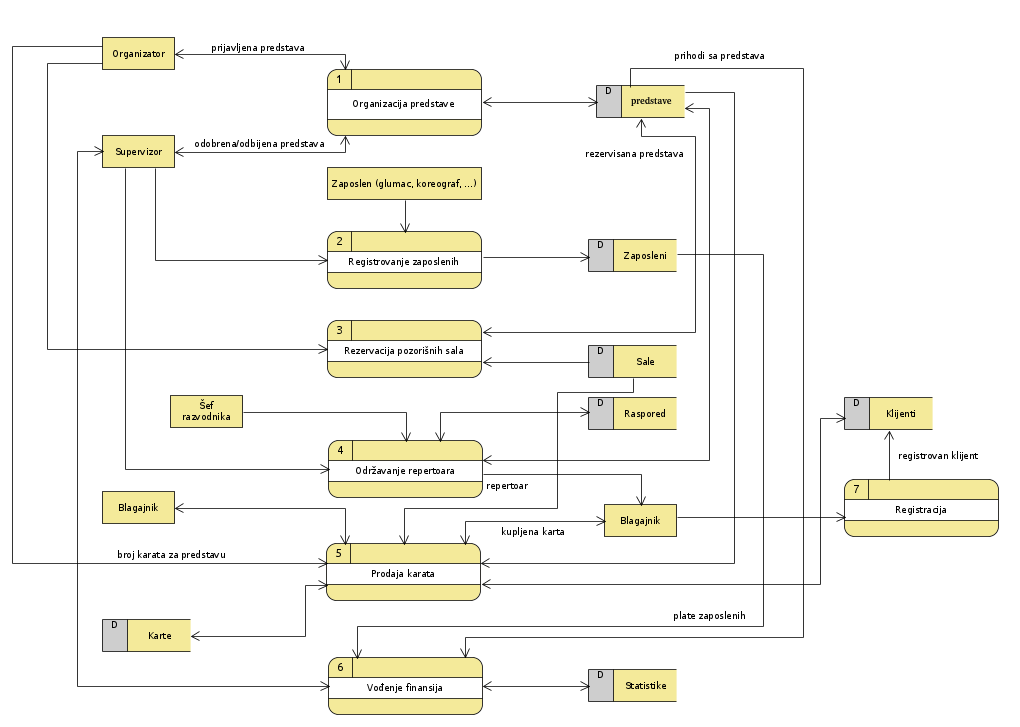
\includegraphics[width=140mm]{../images/dfd1.png}
  \end{center}
  \caption{Dijagram toka podataka prvog nivoa}
  \label{dfd1}
\end{figure}

\section{Slučajevi upotrebe}

\subsection{Organizacija predstave}
Proces organizacije predstave počinje prijavom koju popunjava i podnosi organizator. Predstavu sa statusom ,,prijavljena'' mora da odobri supervizor pozorišta. Kada se prijavljena predstava odobri, onda predstava prelazi u stanje ,,aktivna``. 

Organizator predstave je zadužen za ceo proces formiranja predstave od njene prijave do realizacije, dok supervizor izvršava administrativne zadatke vezane za pozorište. Neophodno je da organizator konstantno ima uvid u stanje svake predstave za koju je on zadužen. 

Pregled procesa je prikazan na slici \ref{usecase_organizacija_predstave}. Prikaz stanja predstave je predstavljen na slici \ref{state_predstava}. Tok podataka pri organizaciji je prikazan dijagramom na slici \ref{dfd2_organizacija_predstave}. 

\begin{figure}[H]
  \begin{center}
      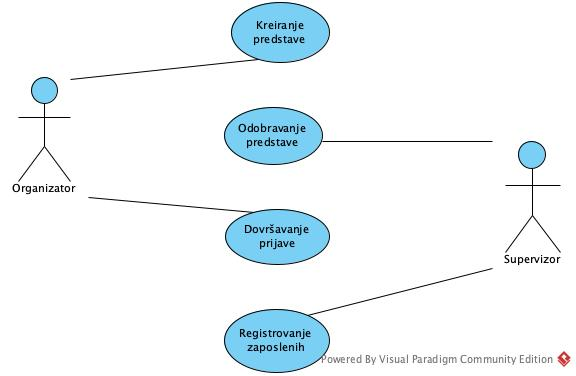
\includegraphics[width=100mm]{../images/usecase_organizacija_predstave.jpg}
  \end{center}
  \caption{Organizacija predstave: dijagram slučaja upotrebe}
  \label{usecase_organizacija_predstave}
\end{figure}

\begin{figure}[H]
  \begin{center}
      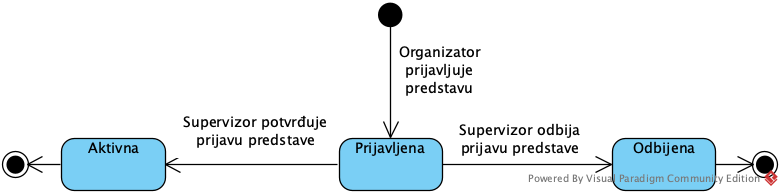
\includegraphics[width=120mm]{../images/state_predstava.png}
  \end{center}
  \caption{Dijagram stanja predstave}
  \label{state_predstava}
\end{figure}

\begin{figure}[H]
  \begin{center}
      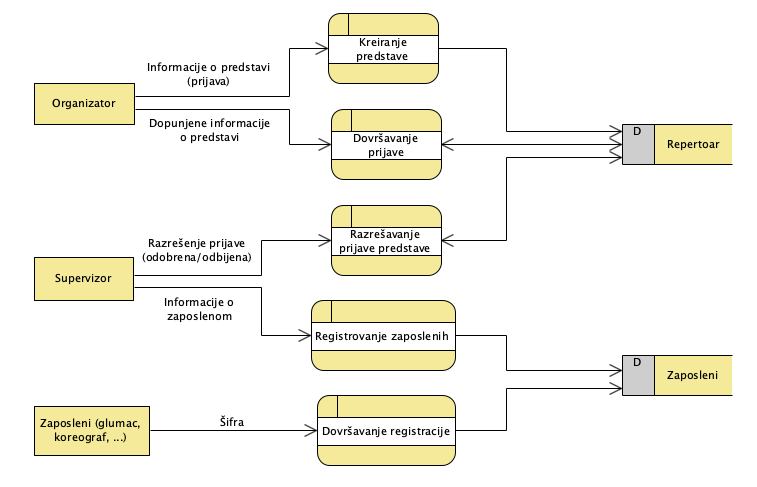
\includegraphics[width=100mm]{../images/dfd2_organizacija_predstave.png}
  \end{center}
  \caption{Organizacija predstave: dijagram toka podataka drugog nivoa}
  \label{dfd2_organizacija_predstave}
\end{figure}

\subsubsection{Kreiranje predstave} \label{Kreiranje predstave}
\noindent\textbf{Kratak opis:} Da bi se predstava održala, organizator mora da je kreira u informacionom sistemu. Aktivnosti pri kreiranju predstave prikazane su na dijagramu \ref{dijagram_aktivnosti_kreiranje_predstave}.

\noindent\textbf{Učesnici:} Organizator predstave

\noindent\textbf{Preduslovi:}
  \begin{itemize}
    \item Postoji zaposleni koji je organizator predstave.
    \item Organizator je prijavljen na sistem.
    \item Postoji scenario za predstavu.
    \item Organizator je ugovorio izvođenje predstave sa rediteljem.
    \item Reditelj je odredio glumce.
    \item Procenjen je budžet koji uključuje platu glumaca tokom pripreme i izvođenja, dužinu pripreme, i elemente scene.
    \item Reditelj i glumci su registrovani u sistemu kao zaposleni.
  \end{itemize}

\noindent\textbf{Postuslovi:} 
  \begin{itemize}
    \item Kreirana predstava je sačuvana u sistemu sa statusom ,,prijavljena``.
    \item Organizator može da vidi prijavljenu predstavu kada je prijavljen na sistem.
  \end{itemize}

\noindent\textbf{Osnovni tok:}
  \begin{legal}
    \item Organizator u sistemu otvara stranu za kreiranje predstave.
    \item Organizator unosi u formu potrebne informacije, uključujući ime i opis predstave, reditelja, glumce i uloge. 
    \item Organizator evidentira prijavu predstave u sistem klikom na ,,Pošalji prijavu``. 
    \item Sistem obaveštava supervizora mejlom o prijavljenoj predstavi.
  \end{legal}

\noindent\textbf{Alternativni tokovi:} 
\begin{itemize}
  \item \textbf{A1. Informacije o prijavi su nepotpune} 
      \begin{legal}
        \item Organizator u koraku 2. ne unosi sve informacije, ili nije siguran da li su informacije finalne. 
        \item Organizator čuva predstavu sa statusom ,,nedovršena'' klikom na ,,Sačuvaj nedovršenu prijavu``.
      \end{legal}
  \item \textbf{A2. Neki od uključenih zaposlenih nije evidentiran u sistemu} 
      \begin{legal}
        \item Organizator ne može da dovrši korak 2 jer jedan od zaposlenih nije evidentiran u sistemu, pa čuva nedovršenu prijavu (Alternativni tok A1)
        \item Supervizor evidentira zaposlenog u sistemu procesom opisanim u \ref{Registrovanje zaposlenih}.
        \item Organizator nastavlja proces kroz \ref{Dovršavanje prijave}
      \end{legal}
\end{itemize}

\noindent\textbf{Dodatne informacije:} Podrazumeva se da je predstava ugovorena drugim putevima - nizom mejlova, telefonskih razgovora i sastanaka. Zbog komplikovane prirode međuljudskih veza u ovoj sferi, informacioni sistem se bavi isključivo ugovorenom predstavom. 

\begin{figure}[H]
  \begin{center}
      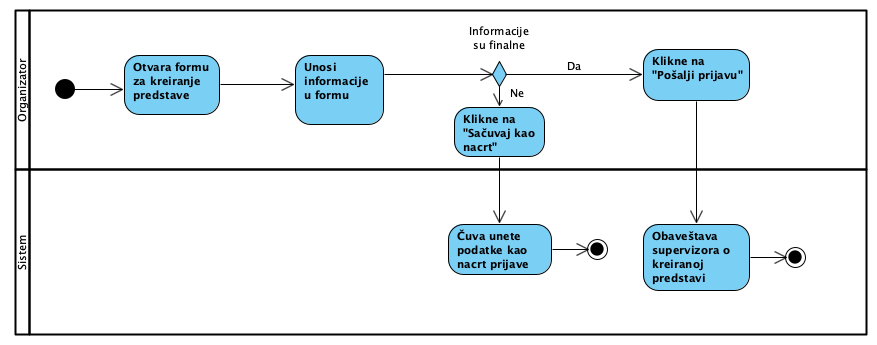
\includegraphics[width=160mm]{../images/dijagram_aktivnosti_kreiranje_predstave.png}
  \end{center}
  \caption{Kreiranje predstave: dijagram aktivnosti}
  \label{dijagram_aktivnosti_kreiranje_predstave}
\end{figure}

\subsubsection{Dovršavanje prijave} \label{Dovršavanje prijave}
\noindent\textbf{Kratak opis:} U slučaju da je organizator sačuvao prijavu kao nedovršenu, može da je izmeni ili dopuni, i konačno pošalje. Aktivnosti pri kreiranju predstave prikazane su na dijagramu \ref{dijagram_aktivnosti_dovrsavanje_prijave}.

\noindent\textbf{Učesnici:} Organizator predstave

\noindent\textbf{Preduslovi:}
  \begin{itemize}
    \item Organizator je prijavljen na sistem.
    \item Organizator je započeo prijavu predstave i sačuvao je kao nedovršenu.
    \item Organizator može da vidi nedovršenu predstavu nakon prijave na sistem.
    \item Svi preduslovi slučaja \ref{Kreiranje predstave}.
  \end{itemize}

\noindent\textbf{Postuslovi:} 
  \begin{itemize}
    \item Predstava koja je bila evidentirana kao ,,nedovršena'' je sada evidentirana kao ,,prijavljena`` .
    \item Svi postuslovi slučaja \ref{Kreiranje predstave}.
  \end{itemize}

\noindent\textbf{Osnovni tok:}
  \begin{legal}
    \item Organizator pretražuje nedovršene prijave.
    \item Organizator otvara određenu nedovšenu prijavu. 
    \item Organizator dopunjava, odnosno menja željene informacije.
    \item Organizator evidentira prijavu predstave u sistem klikom na ,,Pošalji prijavu``. 
    \item Sistem obaveštava supervizora mejlom o prijavljenoj predstavi.
  \end{legal}

\noindent\textbf{Alternativni tokovi:} 
\begin{itemize}
  \item \textbf{A1. Informacije o prijavi su nepotpune} 
      \begin{legal}
        \item Organizator u koraku 2. ne unosi sve informacije, ili nije siguran da li su informacije finalne. 
        \item Organizator čuva predstavu sa statusom ,,nedovršena'' klikom na ,,Sačuvaj nedovršenu prijavu``.
      \end{legal}
\end{itemize}

\begin{figure}[H]
  \begin{center}
      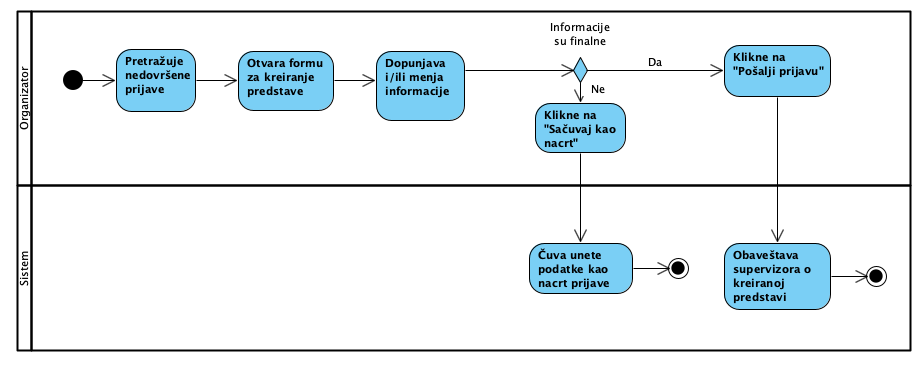
\includegraphics[width=160mm]{../images/dijagram_aktivnosti_dovrsavanje_prijave.png}
  \end{center}
  \caption{Dovršavanje prijave: dijagram aktivnosti}
  \label{dijagram_aktivnosti_dovrsavanje_prijave}
\end{figure}


\subsubsection{Odobravanje predstave}
\noindent\textbf{Kratak opis:} Kada je predstava prijavljena, supervizor pregleda informacije, uzimajući u obzir aktuelni i budući repertoar i interesovanje publike za isti, kao i budžet pozorišta, i odobrava predstavu. Aktivnosti pri odobravanju predstave prikazane su na dijagramu \ref{dijagram_aktivnosti_odobravanje_predstave}.

\noindent\textbf{Učesnici:} Supervizor pozorišta.

\noindent\textbf{Preduslovi:}
  \begin{itemize}
    \item Supervizor je prijavljen na sistem.
    \item Određena predstava je evidentirana u sistemu kao ,,prijavljena``.
  \end{itemize}

\noindent\textbf{Postuslovi:} 
  \begin{itemize}
    \item Predstava koja je bila evidentirana kao ,,prijavljena'' je evidentirana kao ,,aktivna``
    \item Organizator može da vidi odgovarajući status predstave nakon prijave na sistem.
    \item Organizator može da rezerviše sale za probu i održavanje predstave. 
  \end{itemize}

\noindent\textbf{Osnovni tok:}
  \begin{legal}
    \item Supervizor pretražuje predstave sa statusom ,,prijavljena``.
    \item Supervizor otvara stranu za prikaz informacija o određenoj prijavljenoj predstavi. 
    \item Nakon analize informacija, supervizor odobrava predstavu. 
    \item Sistem obaveštava organizatora mejlom o odobrenju. 
  \end{legal}

\noindent\textbf{Alternativni tokovi:} 
\begin{itemize}
  \item \textbf{A1. Predstava je odbijena} 
      \begin{legal}
        \item Supervizor u 3. koraku odbija prijavu predstave uz obrazloženje.
        \item Sistem obaveštava organizatora mejlom o odbijanju uz obrazloženje. 
      \end{legal}
\end{itemize}

\begin{figure}[H]
  \begin{center}
      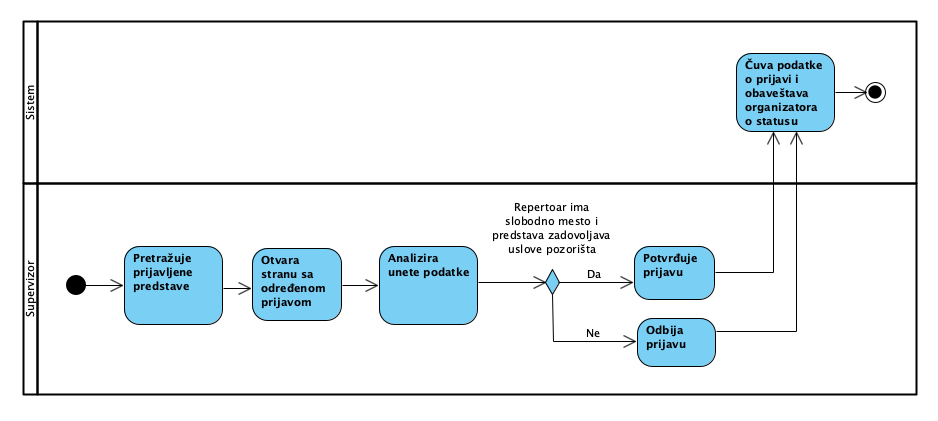
\includegraphics[width=160mm]{../images/dijagram_aktivnosti_odobravanje_predstave.png}
  \end{center}
  \caption{Odobravanje predstave: dijagram aktivnosti}
  \label{dijagram_aktivnosti_odobravanje_predstave}
\end{figure}

\subsubsection{Registrovanje zaposlenog} \label{Registrovanje zaposlenih}
\noindent\textbf{Kratak opis:} Da bi zaposleni bio uključeni u predstavu, mora biti registrovan u sistemu. Supervizor po sklapanju ugovora o radu sa zaposlenim unosi njegove informacije u sistem. Aktivnosti pri registrovanju zaposlenog prikazane su na dijagramu \ref{dijagram_aktivnosti_registrovanje_zaposlenog}.

\noindent\textbf{Učesnici:} Supervizor pozorišta; zaposleni.

\noindent\textbf{Preduslovi:}
  \begin{itemize}
    \item Supervizor je prijavljen na sistem.
    \item Pozorište je sklopilo ugovor o radu sa osobom A.
  \end{itemize}

\noindent\textbf{Postuslovi:} 
  \begin{itemize}
    \item Zaposleni je eveidentiran u sistemu.
    \item Zaposleni može da se prijavi na sistem.
  \end{itemize}

\noindent\textbf{Osnovni tok:}
  \begin{legal}
    \item Supervizor otvara formu za evidentiranje zaposlenog.
    \item Supervizor popunjava formu, unoseći sve potrebne informacije uključujući Ime, Prezime, JMBG i mejl adresu. 
    \item Sistem obaveštava zaposlenog o kreiranom profilu putem mejla. 
    \item Zaposleni klikom na link u mejlu koji mu je stigao odlazi na stranicu gde kreira šifru za svoj nalog i potvrđuje registraciju.  
    \item Sistem čuva unete podatke i obaveštava zaposlenog mailom o uspešnoj registraciji
  \end{legal}

\noindent\textbf{Alternativni tokovi:} 
\begin{itemize}
  \item \textbf{A1. Zaposleni ne potvrđuje registraciju} 
      \begin{legal}
        \item Zaposleni nije ispunio 4. korak. Zaposleni ne može da se prijavi na sistem ali može da bude uključen u prijavu predstave. 
      \end{legal}
\end{itemize}

\begin{figure}[H]
  \begin{center}
      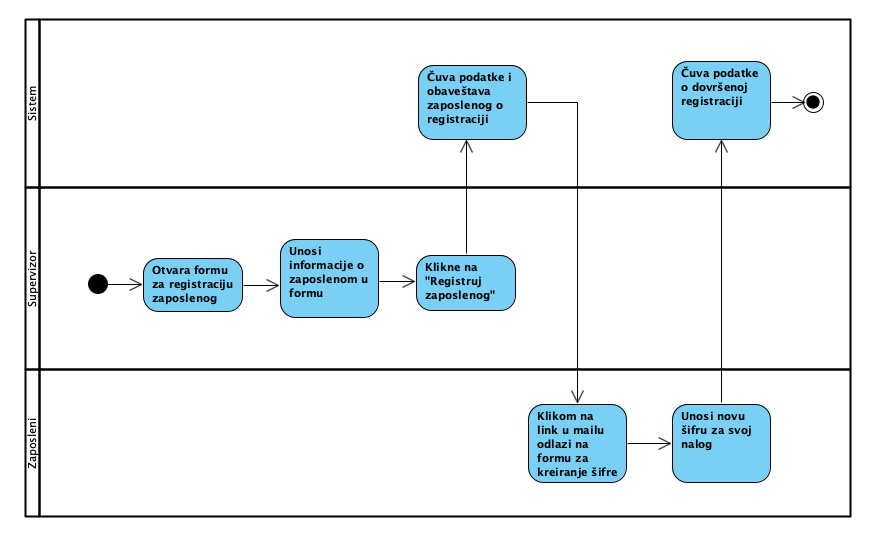
\includegraphics[width=160mm]{../images/dijagram_aktivnosti_registrovanje_zaposlenog.png}
  \end{center}
  \caption{Registrovanje zaposlenog: dijagram aktivnosti}
  \label{dijagram_aktivnosti_registrovanje_zaposlenog}
\end{figure}


% --------------------------------------------------------------------------------------------------

\subsection{Rezervacija pozorišnih sala}
Organizator ima uvid u predstave za koje je zadužen. Nakon organizovanja predstave, i odobravanja iste od strane supervizora, potrebno je rezervisati salu u kojoj će se predstava održati. Pored rezervacije, potrebno je omogućiti  promenu i odjavljivanje sale. Neophodno je da organizator ima uvid u predstave za koje je on zadužen, kao i uvid u slobodne sale za termin održavanja predstave. Za svaku predstavu definisano je datum, vreme i trajanje predstave.

\begin{figure}[H]
  \begin{center}
      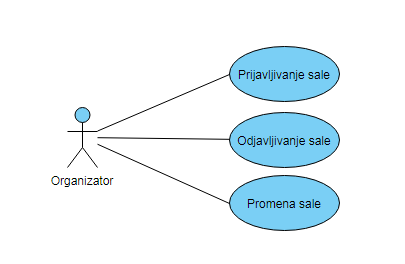
\includegraphics[width=100mm]{../images/usecase_rezervacija_sale.png}
  \end{center}
  \caption{Rezervacija sale: slučaj upotrebe}
  \label{usecase_rezervacija_sale}
\end{figure}

\begin{figure}[H]
  \begin{center}
      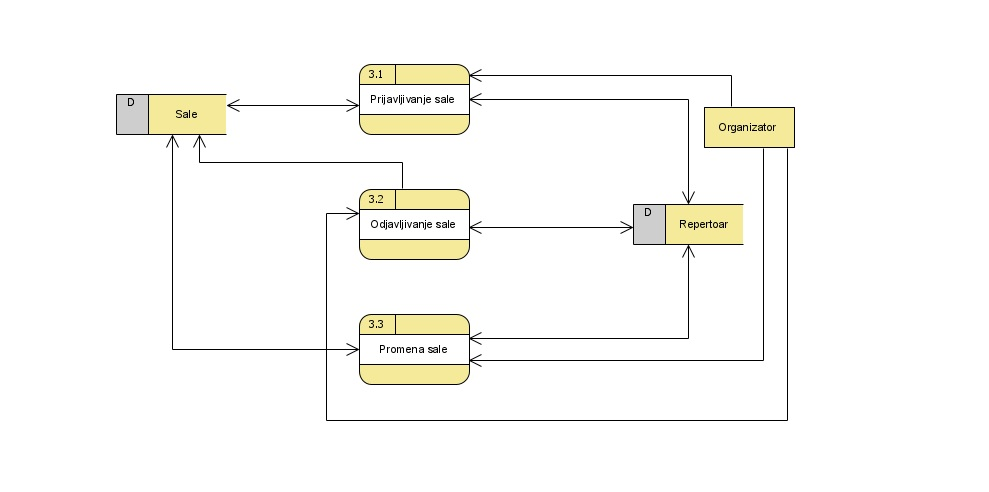
\includegraphics[width=160mm]{../images/dfd2_rezervisanje_sala.jpg}
  \end{center}
  \caption{Rezervacija sale: dijagram toka podataka drugog nivoa}
  \label{dfd2_rezervisanje_sala}
\end{figure}

\begin{figure}[H]
  \begin{center}
      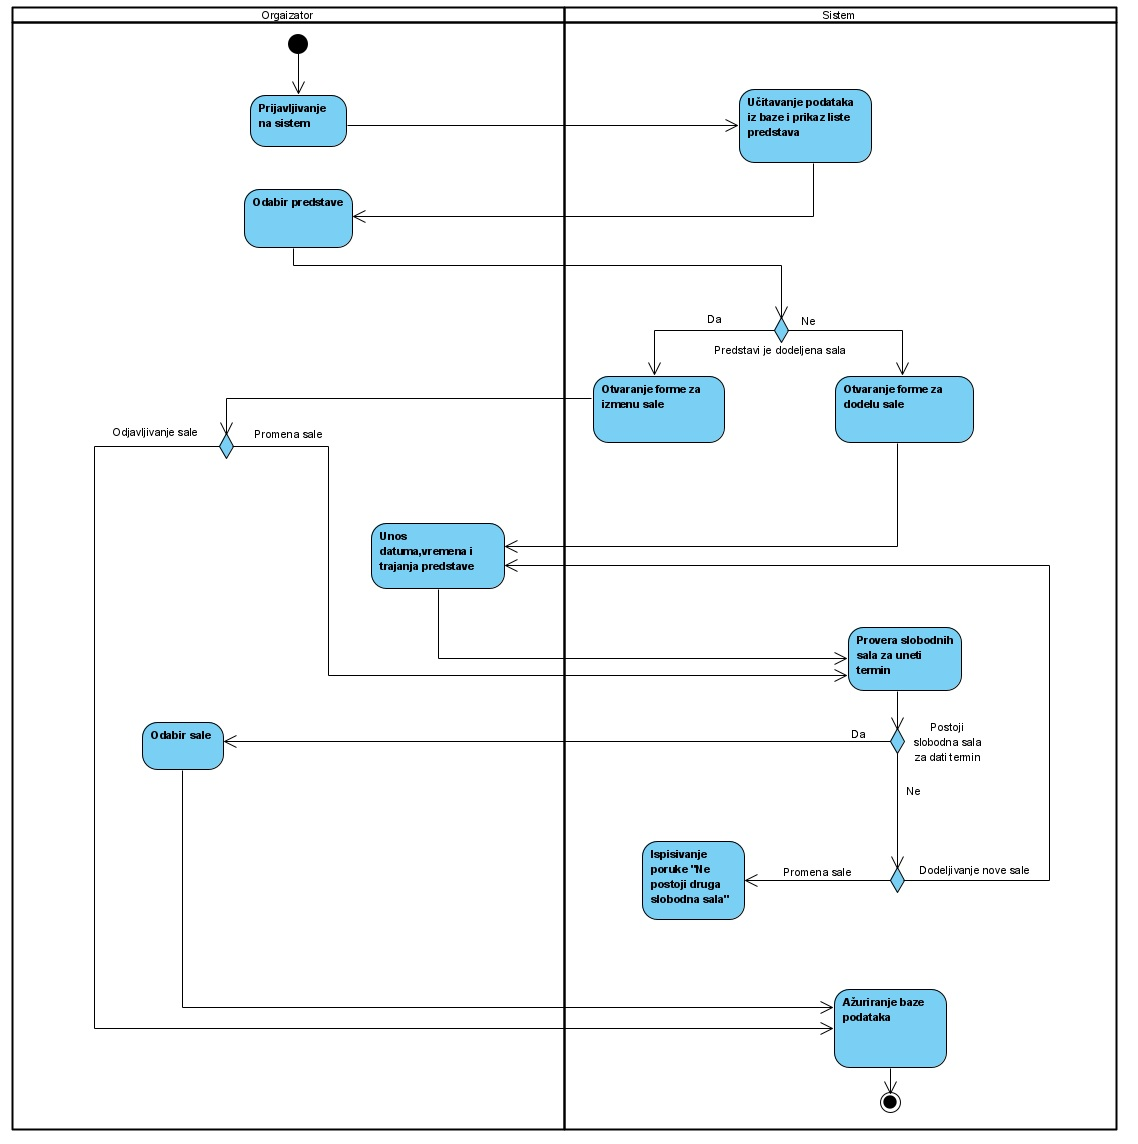
\includegraphics[width=160mm]{../images/activity_rezervacija_sala.jpg}
  \end{center}
  \caption{Rezervacija sale: dijagram aktivnosti}
  \label{activity_rezervacija_sala}
\end{figure}

\subsubsection{Prijavljivanje sale}
\noindent\textbf{Kratak opis:} Kada je predstava odobrena, organizator rezerviše salu za određeni datum i vreme za održavanja predstave. 

\noindent\textbf{Učesnici:} Organizator pozorišta.

\noindent\textbf{Preduslovi:}
  \begin{itemize}
    \item Određena predstava je evidentirana u sistemu kao ,,aktivna``.
  \end{itemize}

\noindent\textbf{Postuslovi:} 
  \begin{itemize}
    \item Sala za održavanje predstave je rezervisana za određeni datum i vreme
    \item Organizator i glumci imaju uvid u kojoj se sali održava predstava nakon prijave na sistem.
  \end{itemize}

\noindent\textbf{Osnovni tok:}
  \begin{legal}
 \item Organizator unosi podatke za prijavljivanje na sistem.
    \item Sistem vrši verifikaciju i prikazuje organizatoru listu predstava za koje je zadužen.
    \item Organizator bira predstavu sa statusom ,,aktivna`` kojoj želi da dodeli salu.
    \item Sistem prikazuje informacije o predstavi.
    \item Organizator unosi datum i vreme održavanja, kao i trajanje predstave
    \item Sistem prikazuje slobodne sale za dati termin.
    \item Organizator dodeljuje slobodnu salu datoj predstavi za određeni termin.
    \item Sistem ažurira bazu podataka.
  \end{legal}

\noindent\textbf{Alternativni tokovi:} 
\begin{itemize}
 \item \textbf{A1. Neuspelo prijavljivanje} 
      \begin{legal}
        \item Sistem prikazuje poruku o grešci pri prijavljivanju.
        \item Proces se nastavlja u \textbf{koraku 1}.
      \end{legal}
  \item \textbf{A7. Sve sale su zauzete za odabrani termin} 
    \begin{legal}
      \item Sistem prikazuje poruku da su sve sale zauzete za dati termin.
      \item Proces se nastavlja u \textbf{koraku 5}.
    \end{legal}
\end{itemize}
\begin{figure}[H]
  \begin{center}
      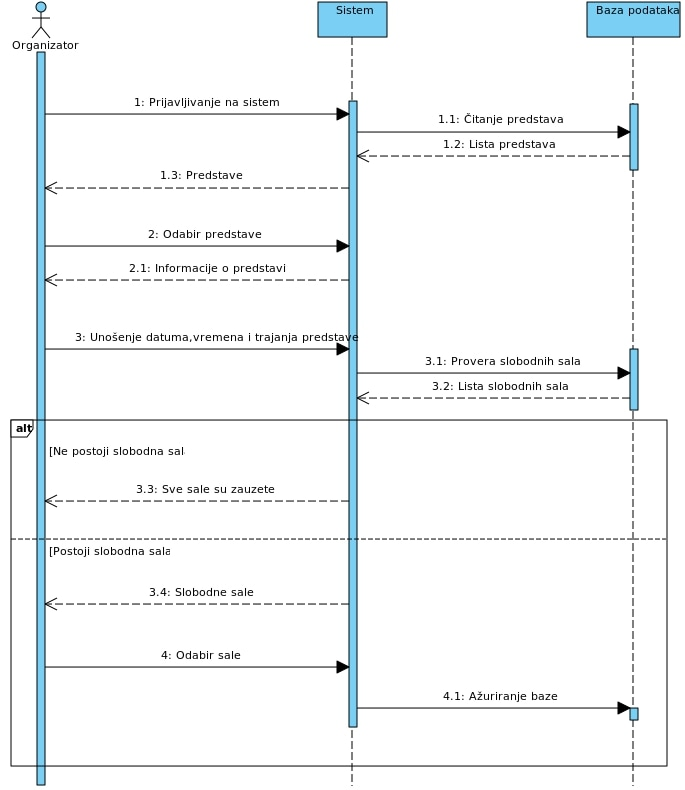
\includegraphics[width=90mm,height=90mm]{../images/sequence_prijavljivanje_sale.jpg}
  \end{center}
  \caption{Prijavljivanje sale: dijagram sekvenci}
  \label{sequence_prijavljivanje_sale}
\end{figure}
\subsubsection{Odjavljivanje sale}
\noindent\textbf{Kratak opis:} Predstava je odložena i organizator odjavljuje datu salu

\noindent\textbf{Učesnici:} Organizator pozorišta.

\noindent\textbf{Preduslovi:}
  \begin{itemize}
    \item Predstavi je dodeljena sala
  \end{itemize}

\noindent\textbf{Postuslovi:} 
  \begin{itemize}
    \item Sala je oslobođena za dati termin
    \item Predstavi nije dodeljena nijedna sala
  \end{itemize}

\noindent\textbf{Osnovni tok:}
  \begin{legal}
   \item Organizator unosi podatke za prijavljivanje na sistem.
    \item Sistem vrši verifikaciju i prikazuje organizatoru listu predstava za koje je zadužen.
    \item Organizator bira predstavu kojoj je dodeljena sala.
    \item Sistem prikazuje informacije o predstavi.
    \item Organizator odjavljuje salu za dati termin.
    \item Sistem ažurira bazu podataka.
  \end{legal}

\noindent\textbf{Alternativni tokovi:} 
\begin{itemize}
 \item \textbf{A1. Neuspelo prijavljivanje} 
      \begin{legal}
        \item Sistem prikazuje poruku o grešci pri prijavljivanju.
        \item Proces se nastavlja u \textbf{koraku 1}.
      \end{legal}
  
\end{itemize}


\subsubsection{Promena sale}
\noindent\textbf{Kratak opis:} Organizator može da promeni salu za održavanje predstave ukoliko je zbog velikog interesovanja gledalaca potrebna sala sa većim kapacitetom

\noindent\textbf{Učesnici:} Organizator pozorišta.

\noindent\textbf{Preduslovi:}
  \begin{itemize}
    \item Predstavi je dodeljena sala
  \end{itemize}

\noindent\textbf{Postuslovi:} 
  \begin{itemize}
    \item Predstavi je promenjena  sala za održavanje
    \item Prvobitno izabrana sala je oslobođena za dati termin
  \end{itemize}

\noindent\textbf{Osnovni tok:}
  \begin{legal}
  \item Organizator unosi podatke za prijavljivanje na sistem.
    \item Sistem vrši verifikaciju i prikazuje organizatoru listu predstava za koje je zadužen.
    \item Organizator bira predstavu kojoj je dodeljena sala.
    \item Sistem prikazuje informacije o predstavi.
    \item Organizator bira opciju za promenu sale
    \item Sistem prikazuje slobodne sale za dati termin.
    \item Organizator dodeljuje slobodnu salu datoj predstavi za određeni termin.
     \item Sistem ažurira bazu podataka.
  \end{legal}

\noindent\textbf{Alternativni tokovi:} 
\begin{itemize}
 \item \textbf{A1. Neuspelo prijavljivanje} 
      \begin{legal}
        \item Sistem prikazuje poruku o grešci pri prijavljivanju..
        \item Proces se nastavlja u \textbf{koraku 1}.
      \end{legal}
       \item \textbf{A6. Sve sale su zauzete za odabrani termin} 
    \begin{legal}
      \item Sistem prikazuje poruku da su sve sale zauzete za dati termin.
      \item Slučaj upotrebe se ovde završava
    \end{legal}
\end{itemize}

% ----------------------------------------------------------------------------------------------------------

\newpage
\subsection{Održavanje repertoara}
  Supervizor treba nedelju dana unapred da proverava da li je došlo do promene repertoara (otkazivanja predstave) i reguliše održavanje gostovanja (u smislu uklapanja u repertoar), dok šef razvodnika treba da napravi raspored rada razvodnika u zavisnosti od repertoara. 
  
  
\begin{figure}[H]
  \begin{center}
      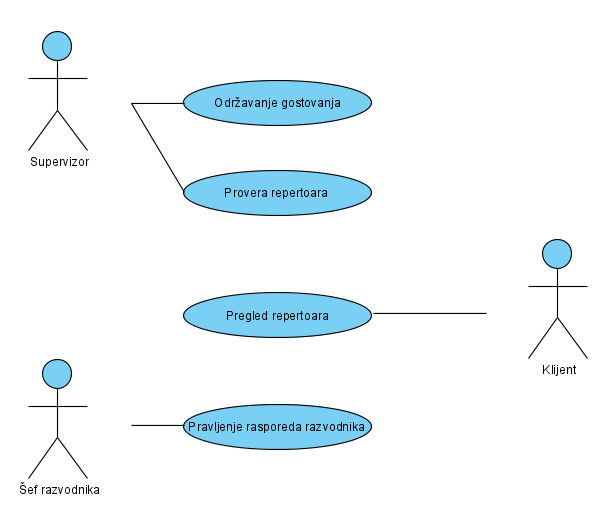
\includegraphics[width=100mm,height=60mm]{../images/usecase_odrzavanje_repertoara.png}
  \end{center}
  \caption{Održavanje repertoara: dijagram slučajeva upotrebe}
  \label{usecase_odrzavanje_repertoara}
\end{figure}

\begin{figure}[H]
  \begin{center}
      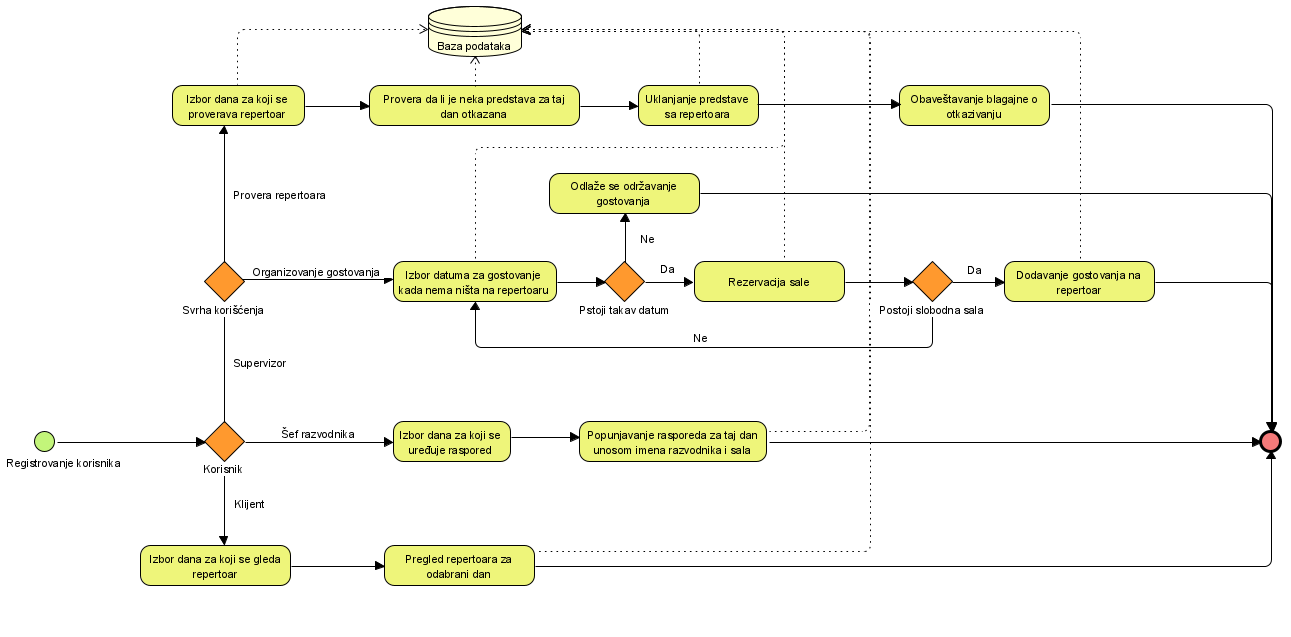
\includegraphics[width=160mm]{../images/bpmn_odrzavanje_repertoara.png}
  \end{center}
  \caption{Održavanje repertoara: BPMN dijagram}
  \label{bpmn_odrzavanje_repertoara}
\end{figure}

\begin{figure}[H]
  \begin{center}
      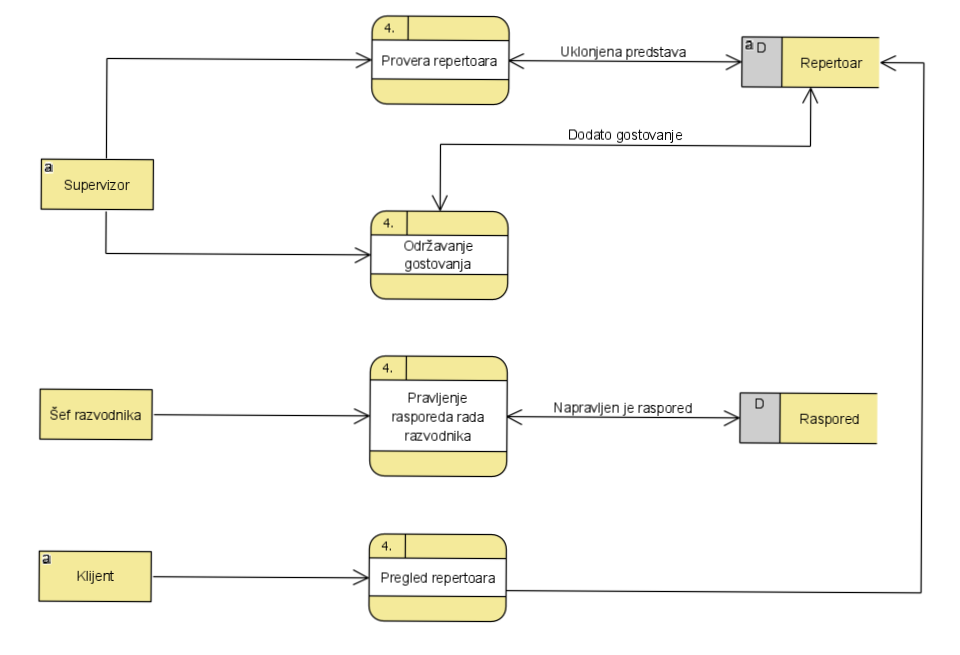
\includegraphics[width=120mm,height=80mm]{../images/dfd2_odrzavanje_repertoara.png}
  \end{center}
  \caption{Održavanje repertoara: dijagram toka podataka drugog nivoa}
  \label{dfd2_odrzavanje_repertoara}
\end{figure}


\subsubsection{Provera repertoara} 
\noindent\textbf{Kratak opis:} Supervizor svakog dana proverava predstave koje su na repertoaru istog dana sledeće nedelje, za slučaj da je neka otkazana.

\noindent\textbf{Učesnici:} Supervizor pozorišta.

\noindent\textbf{Preduslovi:}
  \begin{itemize}
    \item Poznat je repertoar.
    \item Supervizor ima pristup sistemu.
  \end{itemize}

\noindent\textbf{Postuslovi:} 
  \begin{itemize}
    \item Vidljive su izmene u repertoaru.
  \end{itemize}

\noindent\textbf{Osnovni tok:}
  \begin{legal}
    \item Supervizor otvara formu za evidentiranje zaposlenog.
    \item Sistem vrši verifikaciju i prikazuje supervizoru listu datuma koji čine repertoar.
    \item Supervizor bira datum iz te liste koji predstavlja isti dan sledeće nedelje.
    \item Sistem prikazuje informacije za odabrani datum.
    \item Ukoliko postoji problem oko izvođenja predstave (predstava mora da bude otkazana), supervizor uklanja predstavu sa repertoara.
    \item Sistem ažurira bazu podataka.
    \item Supervizor želi da obavesti blagajnu da je predstava otkazana, kako bi rešili probleme sa kartama za otkazanu predstavu.
    \item Sistem obaveštava blagajnu.
  \end{legal}

\begin{figure}[H]
  \begin{center}
      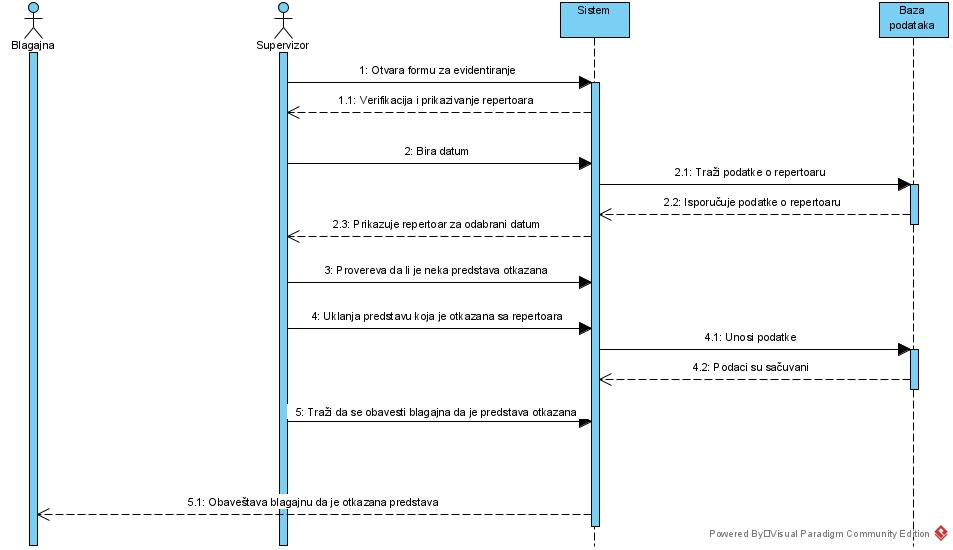
\includegraphics[width=100mm,height=60mm]{../images/sequence_provera_repertoara.jpg}
  \end{center}
  \caption{Provera repertoara: dijagram sekvenci}
  \label{sequence_provera_repertoara}
\end{figure}

\subsubsection{Održavanje gostovanja} 
\noindent\textbf{Kratak opis:} Supervizor treba da uklopi održavanje gostovanja u repertoar. Kada se održava gostovanje, tog dana ne sme da bude ništa na repertoaru.

\noindent\textbf{Učesnici:} Supervizor pozorišta.

\noindent\textbf{Preduslovi:}
  \begin{itemize}
    \item Poznat je repertoar.
    \item Supervizor ima pristup sistemu.
    \item Supervizor je upoznat sa salom u kojoj treba da se održi gotovanje, datumima koji su u opticaju za održavanje i dužinom trajanja gostovanja.
  \end{itemize}

\noindent\textbf{Postuslovi:} 
  \begin{itemize}
    \item Vidljive su izmene u repertoaru.
  \end{itemize}

\noindent\textbf{Osnovni tok:}
  \begin{legal}
    \item Supervizor otvara formu za evidentiranje zaposlenog.
    \item Sistem vrši verifikaciju i prikazuje supervizoru listu datuma koji čine repertoar.
    \item Supervizor bira datum koji odgovara željenom datumu održavanja gostovanja.
    \item Sistem prikazuje repertoar za taj datum.
    \item Supervizor proverava da li se nešto nalazi na repertoaru tog dana.
    \item Ukoliko je odabrani dan slobodan, supervizor proverava da li je željena sala slobodna.
    \item Ukoliko je sala slobodna, supervizor unosi gostovanje u repertoar.
    \item Ažurirana je baza podataka.
  \end{legal}

\noindent\textbf{Alternativni tokovi:} 
\begin{itemize}
 \item \textbf{A1. Odabrani datum nije slobodan} 
      \begin{legal}
        \item U koraku 5. za odabrani datum se već nalazi nešto na repertoaru.
        \item Supervizor se vraća u korak 3. i bira neki drugi datum.
      \end{legal}
  \item \textbf{A2. Tražena sala nije slobodna} 
      \begin{legal}
        \item U koraku 6. za odabrani datum tražena sala nije slobodna
        \item Supervizor se vraća u korak 3. i bira neki drugi datum.
      \end{legal}
  \item \textbf{A3. Nije moguće održati gostovanje} 
      \begin{legal}
        \item U koraku 3. nije preostao ni jedan datum koji je moguće odabrati za gostovanje.
        \item Supervizor odlaže gostovanje do daljenjeg.
      \end{legal}
\end{itemize}


\subsubsection{Pravljenje rasporeda razvodnika} 
\noindent\textbf{Kratak opis:} Šef razvodnika treba da napravi raspored rada razvodnika u zavisnosti od repertoara.

\noindent\textbf{Učesnici:} Šef razvodnika.

\noindent\textbf{Preduslovi:}
  \begin{itemize}
    \item Poznat je repertoar.
    \item Šef razvodnika ima pristup sistemu.
  \end{itemize}

\noindent\textbf{Postuslovi:} 
  \begin{itemize}
    \item Napravljen je raspored rada razvodnika za svaki dan repertoara.
    
  \end{itemize}

\noindent\textbf{Osnovni tok:}
  \begin{legal}
    \item Šef razvodnika otvara formu za evidentiranje zaposlenog.
    \item Sistem vrši verifikaciju i prikazuje šefu razvodnika repertoar i listu datuma za koje treba da sastavi raspored.
    \item Šef razvodnika bira jedan datum iz liste datuma.
    \item Sistem prikazuje postojeće informacije za odabrani datum.
    \item Šef razvodnika za odabrani datum unosi imena razvodnika i salu u kojoj rade.
    \item Sistem ažurira bazu podataka.
  \end{legal}

\begin{figure}[H]
  \begin{center}
      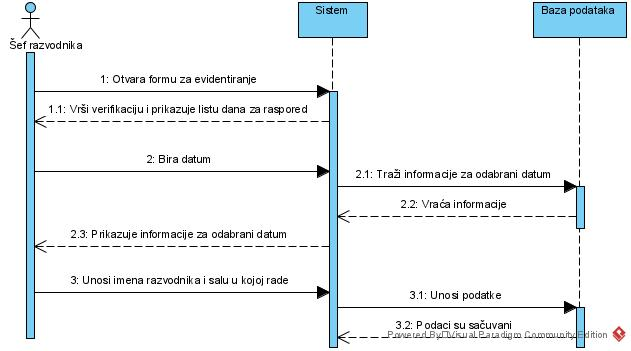
\includegraphics[width=100mm,height=60mm]{../images/sequence_raspored_razvodnika.jpg}
  \end{center}
  \caption{Pravljenje rasporeda razvodnika: dijagram sekvenci}
  \label{sequence_raspored_razvodnika}
\end{figure}

\subsubsection{Pregled repertoara} 
\noindent\textbf{Kratak opis:} Klijent ima mogućnost da pregleda repertoar.

\noindent\textbf{Učesnici:} Klijent

\noindent\textbf{Preduslovi:}
  \begin{itemize}
    \item Poznat je repertoar.
    \item Klijent ima pristup sistemu.
  \end{itemize}

\noindent\textbf{Postuslovi:} 
  \begin{itemize}
    \item Klijent je upoznat sa repertoarom.
  \end{itemize}

\noindent\textbf{Osnovni tok:}
  \begin{legal}
    \item Klijent otvara formu za evidentiranje korisnika.
    \item Sistem vrši verifikaciju i prikazuje klijentu listu datuma koji čine repertoar. 
    \item Klijent bira datum za koji želi da pregleda repertoar.
    \item Sistem prikazuje korisniku spisak predstava koje će se igrati tog dana, zajedno sa vremenom njihovog početka i salom u kojoj se igraju.
  \end{legal}
% ---------------------------------------------------------------------------

\newpage
\subsection{Prodaja karata}
Prodaja karata je proces koji sledi nakon što je određen datum, rezervisana sala i dodeljene uloge
zaposlenim. Tada je moguće preciznije odrediti potreban budžet za dalju realizaciju predstave, pa
samim tim i minimalni broj kupljenih karata za izvođenje. Na osnovu rezervisane sale (i potencijalno još 
nekih drugih faktora, kao što je epidemija ili slično) određuje se broj karata za prodaju. Gledaoci 
(klijenti) predstave mogu da kupe ili rezervišu kartu za pozorište preko veb stranice pozorišta. 
Takođe, klijenti mogu da kupe rezervisanu kartu ili nerezervisanu kartu ako nisu rasprodate na blagajni.
Klijent ima pravo da zatraži povraćaj novca za kupljenu kartu, a slučaju da se cela predstava otkaže,
potrebno je, uz potvrdu organizatora, da se izvrši povraćaj novca svim klijentima.

\begin{figure}[H]
  \begin{center}
      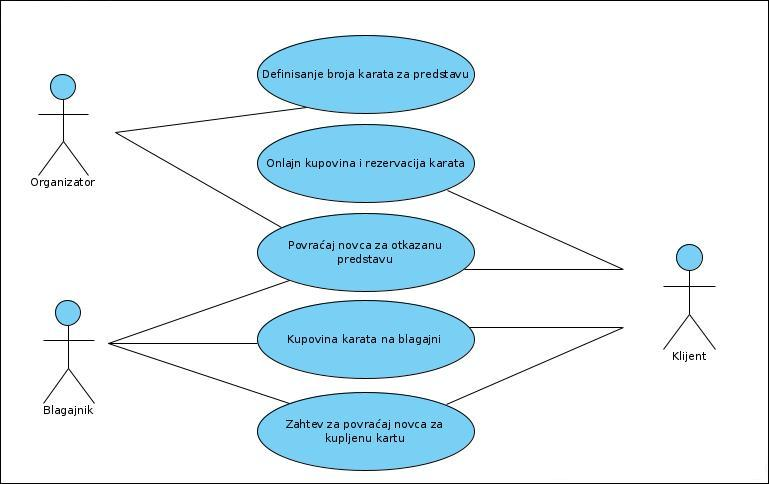
\includegraphics[width=100mm,height=60mm]{../images/usecase_prodaja_karata.jpg}
  \end{center}
  \caption{Prodaja karata: dijagram slučajeva upotrebe}
  \label{usecase_prodaja_karata}
\end{figure}

Ovaj proces ima, grubo rečeno, tri glavna stanja:
\begin{itemize}
  \item Predstava je aktivna;
  \item Kupovina i rezervacija karata;
  \item Povraćaj novca (opcionalno i neželjno stanje).
\end{itemize}

\begin{figure}[H]
  \begin{center}
      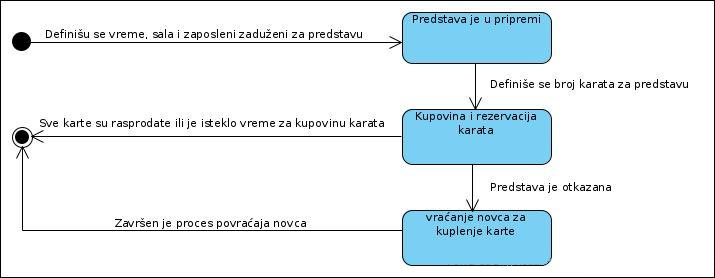
\includegraphics[width=100mm,height=40mm]{../images/state_prodaja_karata.jpg}
  \end{center}
  \caption{Prodaja karata: dijagram stanja}
  \label{state_prodaja_karata}
\end{figure}

Celokupni proces se deli na dve celine: definisanje broja karata za predstavu (organizacija) i trgovina 
kartama. To se i može primetiti na dijagramu toka podataka. Repertoar je neophodan kako zbog čitanja
i ažuriranja broja slobodnih karata za neku konkretnu predstavu, a lista karata je neophodna za čuvanje
kodova rezervisanih i kupljenih karata.  

\begin{figure}[H]
  \begin{center}
      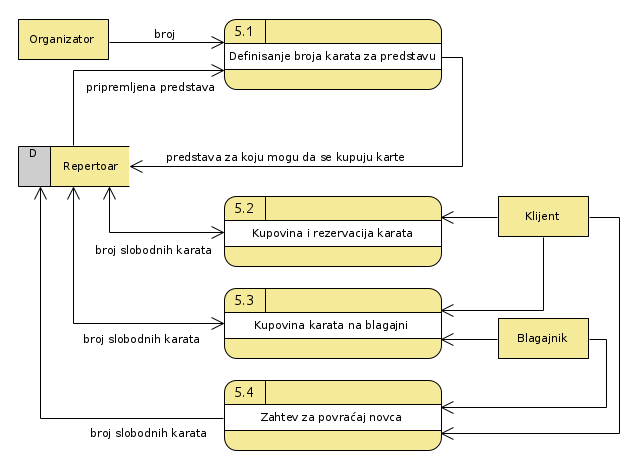
\includegraphics[width=120mm,height=80mm]{../images/dfd2_prodaja_karata.png}
  \end{center}
  \caption{Prodaja karata: dijagram toka podataka drugog nivoa}
  \label{dfd2_prodaja_karata}
\end{figure}

\subsubsection{Definisanje broja karata za predstavu}
\noindent\textbf{Kratak opis:} Organizator predstave može da definiše broj karata na osnovu rezervisane
sale za izvođenje predstave. Nakon definisanja se ažurira repertoar na stranici pozorišta.\\

\noindent\textbf{Učesnici:} Organizator predstave.\\

\noindent\textbf{Preduslovi:}
  \begin{itemize}
    \item Predstava je zakazana određenog datuma.
    \item Rezervisana je određena sala za predstavu.
    \item Dodeljene su sve uloge (tehničke i umetničke) za realizaciju predstave.
    \item Određen je potreban budžet za realizaciju.
    \item Organizator je zadužen za datu predstavu.
  \end{itemize}

\noindent\textbf{Postuslovi:} 
  \begin{itemize}
    \item Ažuriran je repertoar tj. dodata je nova predstava sa kratkim opisom i datumom izvođenja.
    \item Ažuriran je status predstave u bazi podataka.
    \item Korisnici su u mogućnosti da rezervišu ili kupe kartu za tu predstavu.
  \end{itemize}

\noindent\textbf{Osnovni tok:}
  \begin{legal}
    \item Organizator unosi podatke za prijavljivanje na sistem.
    \item Sistem vrši verifikaciju i prikazuje organizatoru listu predstava za koje je on zadužen.
    \item Organizator bira predstavu koju želi da ažurira.
    \item Sistem prikazuje informacije o predstavi.
    \item Organizator unosi broj karata za prodaju i opciono dodaje napomenu.
    \item Sistem proverava unete podatke.
    \item Sistem ažurira bazu podataka.
  \end{legal}

\noindent\textbf{Alternativni tokovi:} 
\begin{itemize}
  \item \textbf{A1. Neuspelo prijavljivanje (korak 1)} 
      \begin{legal}
        \item Sistem prikazuje poruku o grešci pri prijavljivanju..
        \item Proces se nastavlja u \textbf{koraku 1}.
      \end{legal}
  \item \textbf{A2. Podaci o broju karata nisu validni (korak 6)} 
    \begin{legal}
      \item Sistem prikazuje poruku o grešci.
      \item Proces se nastavlja u \textbf{koraku 5}.
    \end{legal}
\end{itemize}

\noindent\textbf{Dodatne informacije:} 
  \begin{itemize}
    \item Postoji period osvežavanja repertoara na stranici na osnovu
          sadržaja baze podataka. 
    \item Sistem automatski popunjava vrednost polja za broj karata sa podrazumevanom
          vrednošću koja odgovara broju mesta u sali u kojoj je predstava zakazana.
  \end{itemize}

\subsubsection{Onlajn kupovina karata i rezervacija}

\noindent\textbf{Kratak opis:} Informacioni sistem nudi pregled repertoara korisnicima. 
        Svako može da kupi kartu za određenu predstavu ako postoji slobodno mesto.
        Alternativa je da se vrši rezervacija karte koja može kasnije da se kupi na blagajni.\\

\noindent\textbf{Učesnici:} Registrovan korisnik koji želi da kupi ili rezerviše kartu.\\

\noindent\textbf{Preduslovi:} 
  \begin{itemize}
    \item Korisnik mora da bude registrovan sa odgovarajućim mejlom. 
    \item Korisnik mora da ima pristup internetu.
    \item Sistem mora da bude u funkciji.
    \item Sistem mora da bude pouzdan. 
    \item Mora da postoji barem jedno slobodno mesto za željenu predstavu, a samim tim mora da 
          postoji barem jedna aktivna predstava. 
    \item Ukoliko korisnik želi da kupi kartu, mora da ima karticu za onlajn plaćanje (ili 
          neku alternativu).
  \end{itemize}
  
\noindent\textbf{Postuslovi:} 
  \begin{itemize}
    \item Korisnik je dobio potvrdu na mejl sa kodom kupljenje ili rezervisane karte.
    \item Ako je korisnik kupio kartu, onda je takođe dobio mejl sa informacijama računa.
    \item Baza je ažurirana tj. broj karata za predstavu je umanjen za broj kupljenih karata.
  \end{itemize}

\noindent\textbf{Osnovni tok:}
  \begin{legal}
    \item Prijavljen korisnik pristupa stranici za kupovinu karata. 
    \item Sistem učitava podatke iz baze i prikazuje repertoar.
    \item Korisnik klikom bira željenu predstavu sa prikazanog repertoara.
    \item Sistem otvara korisniku formu za rezervaciju ili kupovinu karte.
    \item Korisnik kupuje ili rezerviše kartu.
    \item Sistem proverava formu i ažurira bazu podataka.
    \item Sistem šalje mejl sa odgovarajućim kodom korisniku na mejl.
    \item Sistem prikazuje korisniku poruku o uspešnoj kupovili ili registraciji i podseća
          korisnika da proveri mejl.
  \end{legal}

\noindent\textbf{Alternativni tokovi:} 
  \begin{itemize}
    \item \textbf{A1. Korisnik nije prijavljen} 
        \begin{legal}
          \item Sistem otvara korisniku stranicu za prijavljivanje.
          \item Korisnik se prijavljuje.
          \item Proces se nastavlja u \textbf{koraku 2}.
        \end{legal}
    \item \textbf{A2. Korisnik je već rezervisao kartu (korak 5)}
        \begin{legal}
          \item Sistem prikazuje korisniku obaveštenje o nemogućnosti rezervacije više od jedne karte.
          \item Korisnik pretiska dugme za potvrdu.
          \item Proces se nastavlja u \textbf{koraku 2}.
        \end{legal}
    \item \textbf{A3. Neuspešna kupovina karte (korak 5)}
        \begin{legal}
          \item Sistem prikazuje korisniku obaveštenje o neuspelom plaćanju sa odgovarajućim
                razlogom (ako je taj razlog poznat sistemu).
          \item Korisnik pretiska dugme za potvrdu.
          \item Proces se nastavlja u \textbf{koraku 5}.
        \end{legal}
    \item \textbf{A4. Tokom popunjavanja forme su rasprodate karte su se rasprodale (korak 6)}
        \begin{legal}
          \item Sistem prikazuje korisniku obaveštenje o rasprodatim kartama.
          \item Korisnik pretiska dugme za potvrdu.
          \item Proces se nastavlja u \textbf{koraku 2}.
        \end{legal}
  \end{itemize}

\noindent\textbf{Podtokovi:}
  \begin{itemize}
    \item \textbf{5.1. Kupovina karte}
        \begin{legal}
          \item Korisnik bira opciju za kupovinu karte.
          \item Sistem prikazuje korisniku stranicu, gde može da se izabere broj karata.
          \item Korisnik unosi željeni broj karata.
          \item Sistem izračunava cenu i prikazuje tu cenu korisniku.
          \item Korisnik potvrđuje kupovinu karte tako što pretiska dugme.
          \item Sistem prikazuje korisniku opcije plaćanja.
          \item Korisnik bira željeni način plaćanja.
          \item Sistem prikazuje korisniku formu za plaćanje za izabran način plaćanja.
          \item Korisnik popunjava formu.
          \item Korisnik pretiska dugme za potvrdu.
          \item Sistem izvršava transakciju plaćanja sa odgovarajućim proveravama.
        \end{legal}
    \item \textbf{5.2. Rezervacija karte}
        \begin{legal}
          \item Korisnik bira opciju za rezervaciju karte.
          \item Korisnik potvrđuje rezervaciju karte tako što pretiska dugme.
        \end{legal}
  \end{itemize}

\noindent\textbf{Specijalni zahtevi:} Mejl mora da stigne korisniku u roku od 10 minuta nakon što 
        je prikazana poruka o uspešnoj kupovini odnosno rezervaciji.\\

\noindent\textbf{Dodatne informacije:} Podaci koji su potrebni za prijavu su korisničko ime ili mejl, i 
        šifra naloga.

        \newpage
        \begin{figure}[H]
          \begin{center}
              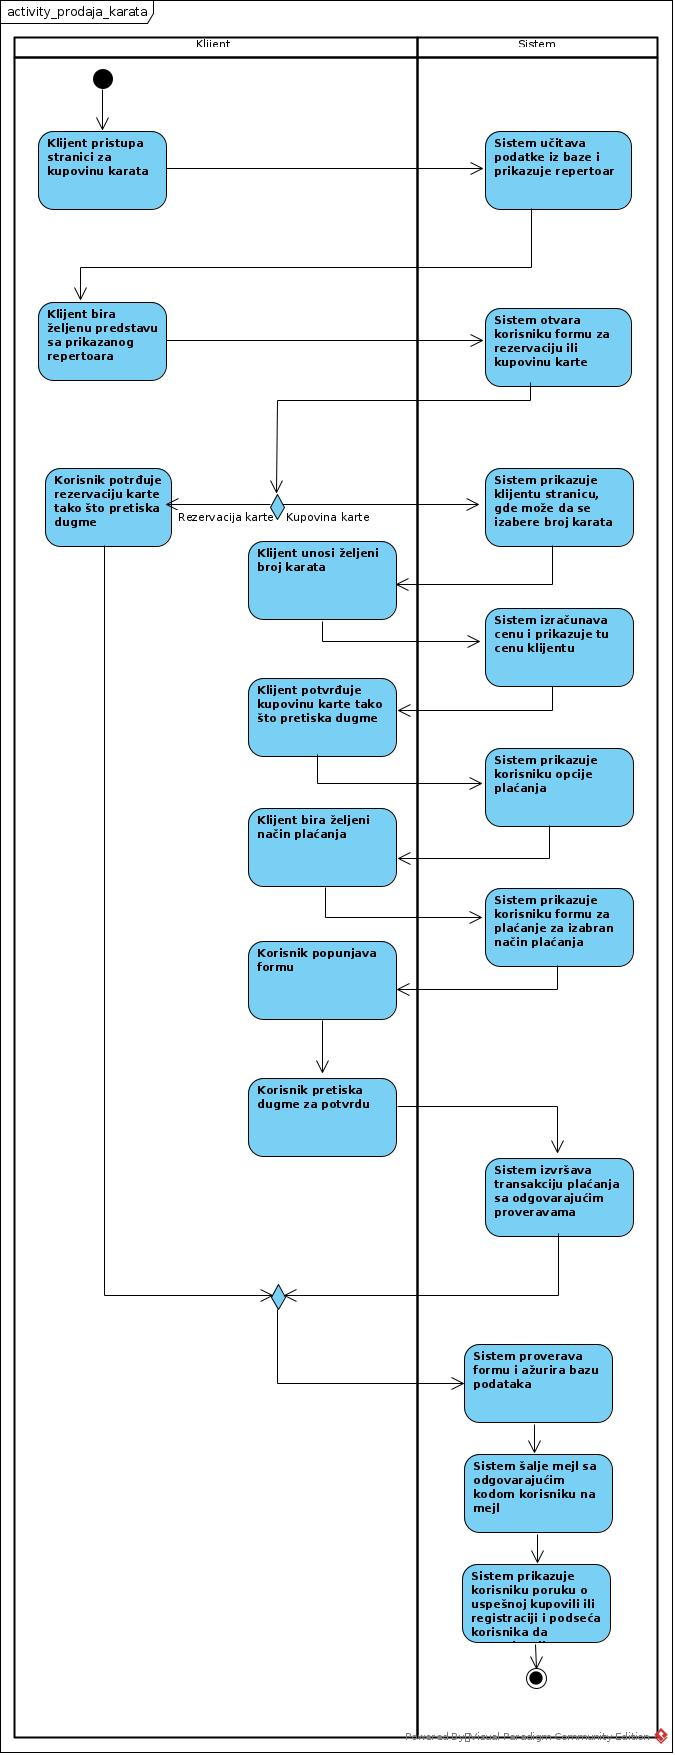
\includegraphics[width=120mm]{../images/activity_prodaja_karata.jpg}
          \end{center}
          \caption{Tok onlajn prodaje karata}
          \label{activity_prodaja_karata}
        \end{figure}

\subsubsection{Kupovina karata na blagajni}
\noindent\textbf{Kratak opis:} Klijenti koji su rezervisali kartu mogu da kupe kartu u pozorištu.
Klijenti koji nisu rezervisali kartu u pozorišu mogu da kupe kartu ako i dalje postoji mesta.\\

\noindent\textbf{Učesnici:} 
  \begin{itemize}
    \item Klijent koji želi da kupi ili rezerviše kartu.
    \item Blagajnik koji je zaposlen u pozorištu.
  \end{itemize}

  \noindent\textbf{Postuslovi:} 
  \begin{itemize}
    \item Klijent ima mogućnost da prisustvuje predstavi za koju ima kupljenu kartu.
  \end{itemize}

  \noindent\textbf{Osnovni tok:}
  \begin{legal}
    \item Klijent saopštava blagajniku koje karte želi da kupi.
    \item Blagajnik zahteva račun za kupovinu od sistema.
    \item Sistem prikazuje prodavcu račun za kupovinu.
    \item Blagajnik saopštava ukupnu cenu klijentu.
    \item Klijent izvršava plaćanje.
    \item Blagajnik potvrđuje uplatu u sistemu.
    \item Sistem prikazuje karte za štampanje.
    \item Blagajnik štampa i daje klijentu karte.
  \end{legal}

  \noindent\textbf{Alternativni tokovi:} 
  \begin{itemize}
    \item \textbf{A1. Ne postoji dovoljan broj karata za brodaju (korak 1.1.2)} 
        \begin{legal}
          \item Blagajnik saopštava klijentu da ne postoji dovoljan broj karata
          \item Proces se nastavlja u \textbf{koraku 1}.
        \end{legal}
    \item \textbf{A2. Kodovi koje je klijent saopštio nisu validni (korak 1.2.2)} 
        \begin{legal}
          \item Blagajnik saopštava klijentu da rezervacije nisu važeće.
          \item Proces se nastavlja u \textbf{koraku 1}.
        \end{legal}
    \item \textbf{A3. Klijent ipak ne želi da izvrši plaćanje (korak 5)} 
        \begin{legal}
          \item Blagajnik stornira račun.
          \item Proces se nastavlja u \textbf{koraku 1}.
        \end{legal}
  \end{itemize}

  \noindent\textbf{Podtokovi:}
  \begin{itemize}
    \item \textbf{1.1. Klijent nema rezervisane karte}
        \begin{legal}
          \item Blagajnik proverava da li ima slobodnih karata tako što unosi upit preko odgovarajućeg interfejsa.
          \item Sistem daje prodavcu informacije o broju slobodnih karata za dati upit.
        \end{legal}
    \item \textbf{1.2. Klijent ima rezervisane karte}
        \begin{legal}
          \item Blagajnik zahteva odgovarajući kod za rezervisane karte.
          \item Kupac daje prodavcu kod za rezervisane karte.
          \item Blagajnik provera da li je kod validan tako što ga unosi u sistem.
          \item Sistem potvrđuje validnost koda.
        \end{legal}
  \end{itemize}

\noindent\textbf{Dodatne informacije:} Ukoliko klijenti ne kupe rezervisane karte do nekog roka (pred početak predstave),
gube se rezervacije i time se povećava broj slobodnih karata.

\begin{figure}[H]
  \begin{center}
      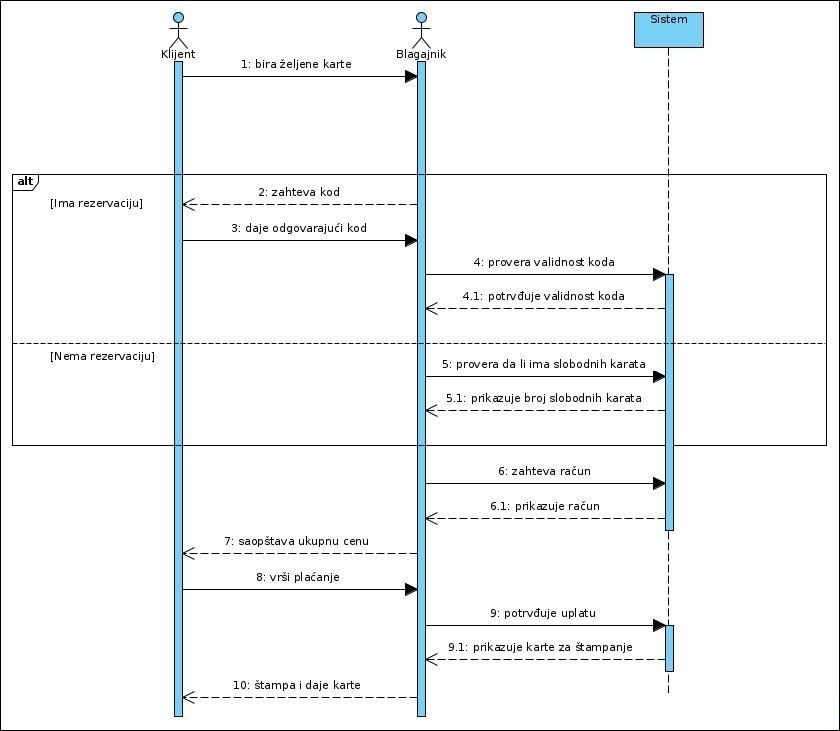
\includegraphics[width=120mm]{../images/sequence_prodaja_karata.jpg}
  \end{center}
  \caption{Prodaja karata na blagajni: dijagram sekvenci}
  \label{sequence_prodaja_karata}
\end{figure}


\subsubsection{Zahtev za povraćaj novca za kupljenu kartu}  
\noindent\textbf{Kratak opis:} Korisnik može da zahteva povraćaj novca za kupljenu kartu neke predstave.
\noindent\textbf{Učesnici:} 
  \begin{itemize}
    \item Klijent koji zahteva povraćaj novca.
    \item Blagajnik koji je zaposlen u pozorištu.
  \end{itemize}

  \noindent\textbf{Preduslovi:} 
  \begin{itemize}
    \item Korisnik je prethodno kupio kartu.
    \item Predstava nije još održana.
  \end{itemize}

  \noindent\textbf{Postuslovi:} 
  \begin{itemize}
    \item Ako je zahtev za povraćaj novca prihvaćen, onda je klijentu povraćen novac.
  \end{itemize}

  \noindent\textbf{Osnovni tok:}
  \begin{legal}
    \item Klijent saopštava blagajniku da želi povraćaj novca.
    \item Blagajnik zahteva od sistema informacije o povraćaju novca za datu kartu.
    \item Sistem prikazuje informacije.
    \item Blagajnik odgovara na zahtev klijenta.
  \end{legal}

  \noindent\textbf{Podtokovi:}
  \begin{itemize}
    \item \textbf{4.1. Zahtev za povraćaj novca je moguć}
        \begin{legal}
          \item Blagajnik saopštava klijentu ponudu za povraćaj novca.
          \item Klijent prihvata ponudu. 
          \item Blagajnik šalje zahtev sistemu za povraćaj novca.
          \item Sistem ažurira bazu podataka, gde je broj slobodnih karata povećava.
          \item Sistem obaveštava blagajnika da je operacija uspešna.
          \item Blagajnik isplaćuje klijentu novac.
        \end{legal}
    \item \textbf{4.2. Zahtev za povraćaj novca nije moguć}
        \begin{legal}
          \item Blagajnik saopštava klijentu da povraćaj novca nije moguć.
        \end{legal}
  \end{itemize}

  \noindent\textbf{Alternativni tokovi:} 
  \begin{itemize}
    \item \textbf{A1. Klijentu ne odgovara ponuda za povraćaj novca (korak 4.1.2)} 
        \begin{legal}
          \item Klijent saopštava blagajniku da ne prihvata ponudu.
          \item Proces se završava.
        \end{legal}
    \item \textbf{A2. Neuspeo povraćaj novca (korak 4.1.4)} 
        \begin{legal}
          \item Blagajnik saopštava klijenta da povraćaj novca trenutno nije moguć.
          \item Proces se završava.
        \end{legal}
  \end{itemize}

  \noindent\textbf{Dodatne informacije:} 
  \begin{itemize}
    \item Pri povraćaju novca za kartu, sistem prikazuje procenat novca
  koji se vraća. Primer: Za kupljenu kartu se vraća 50\% od inicijalne cene. Procenat obračunava sistem
  na osnovu prethodno definisanih pravila.
    \item Ukoliko klijent zahteva novac za otkazanu predstavu, procenat novca koji se vraća je 100\%.
  \end{itemize}

  \begin{figure}[H]
    \begin{center}
        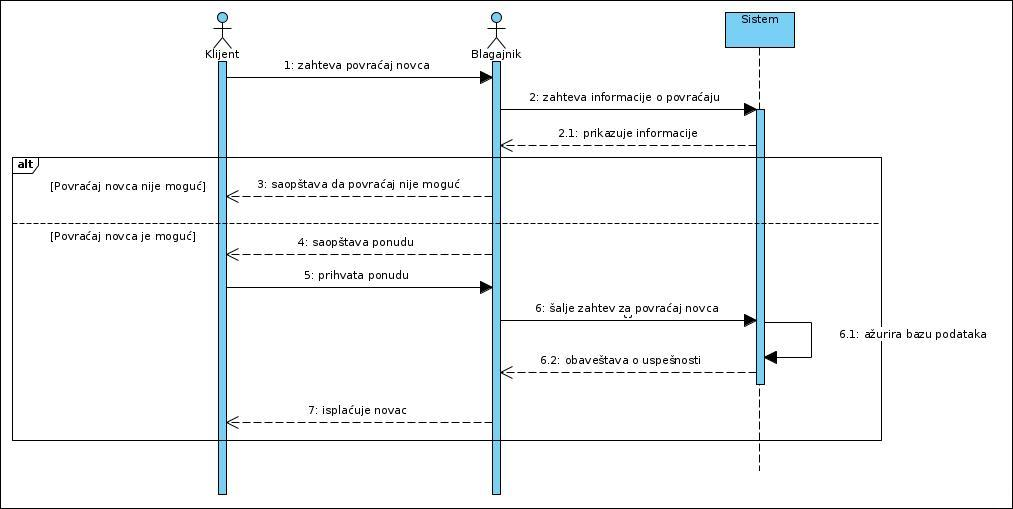
\includegraphics[width=120mm,height=70mm]{../images/sequence_povracaj_novca.jpg}
    \end{center}
    \caption{Povraćaj novca: dijagram sekvenci}
    \label{sequence_povracaj novca}
  \end{figure}

% -------------------------------------------------------------------------------------------------------

\subsection{Vođenje finansija}

 \noindent\textbf{Kratak opis:} Supervizor pozorišta može da vidi prilive i odlive za ceo sistem ili
        neku konkretnu predstavu. 

\begin{figure}[H]
  \begin{center}
      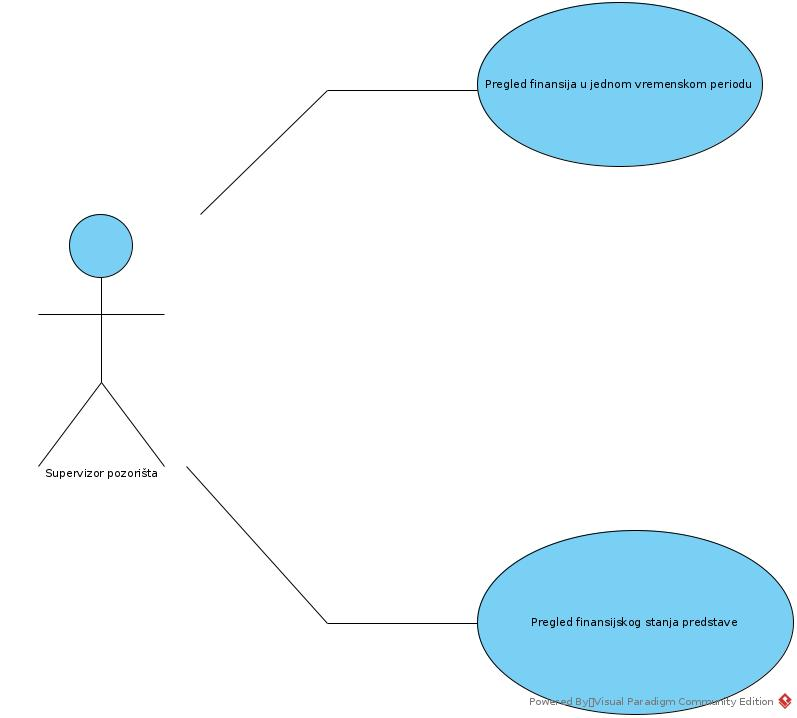
\includegraphics[width=100mm,height=60mm]{../images/usecase_vodjenje_finansija.jpg}
  \end{center}
  \caption{Vođenje finansija: dijagram slučaja upotrebe}
  \label{usecase_vodjenje_finansija}
\end{figure}

\begin{figure}[H]
  \begin{center}
      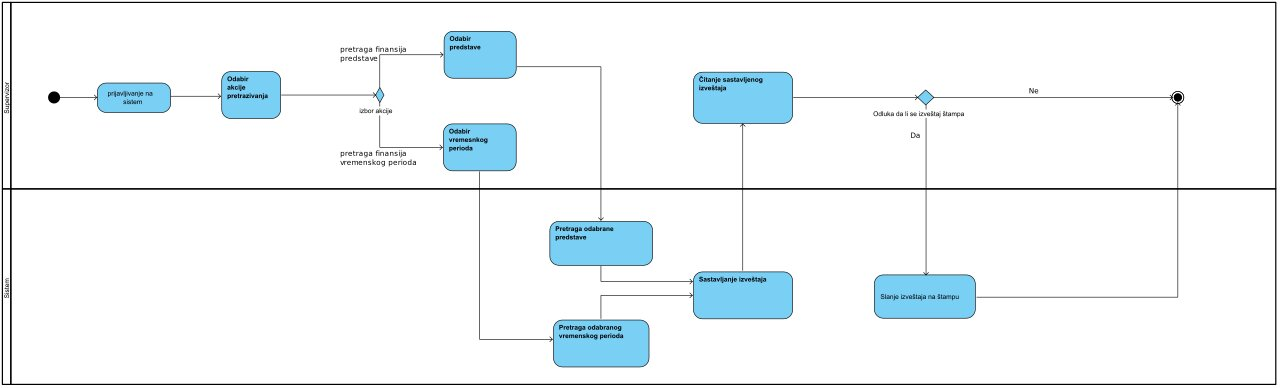
\includegraphics[width=140mm,height=50mm]{../images/activity_vodjenje_finansija.jpg}
  \end{center}
  \caption{Vođenje finansija: objedinjeni dijagram aktivnosti}
  \label{activity?vodjenje?finansija}
\end{figure}

\subsubsection{Pregled finansija u određenom vremenskom periodu}
\noindent\textbf{Kratak opis:} Supervizor pozorišta može zatražiti pregled finansija
u određenom vremenskom periodu. Nakon što dobije prikaz izveštaja, on ima opciju da izveštaj
odštampa ili sačuva na sistemu.

\noindent\textbf{Učesnici:} 
\begin{itemize}
  \item Supervizor pozorišta
\end{itemize}

\noindent\textbf{Preduslovi:} 
\begin{itemize}
  \item Supervizor pozorišta je prijavljen na sistem
\end{itemize}

\noindent\textbf{Postuslovi:} 
\begin{itemize}
  \item Supervizor je obavešten o svim finansijskim informacijama u traženom vremenskom periodu
\end{itemize}

\noindent\textbf{Osnovni tok:} 
\begin{legal}
  \item Supervizor u sistemu otvara stranu za pregled finansija
  \item Supervizor unosi vremenski period za koji zahteva pregled finansija
  \item Sistem prikazuje podatke o finansijama za uneti period
  \item Supervizor bira da li štampa izveštaj
\end{legal}

\noindent\textbf{Alternativni tokovi:}
\begin{itemize}
  \item \textbf{A1. Ne postoje podaci o traženom vremenskom periodu (korak 2)} 
      \begin{legal}
        \item Sistem obaveštava supervizora o problemu
        \item Proces se nastavlja u \textbf{koraku 1}.
      \end{legal}

  \item \textbf{A2. Štampač nije dostupan (korak 4)} 
    \begin{legal}
      \item Sistem obaveštava supervizora o problemu
      \item Proces se završava
    \end{legal}
\end{itemize}

\begin{figure}[H]
  \begin{center}
    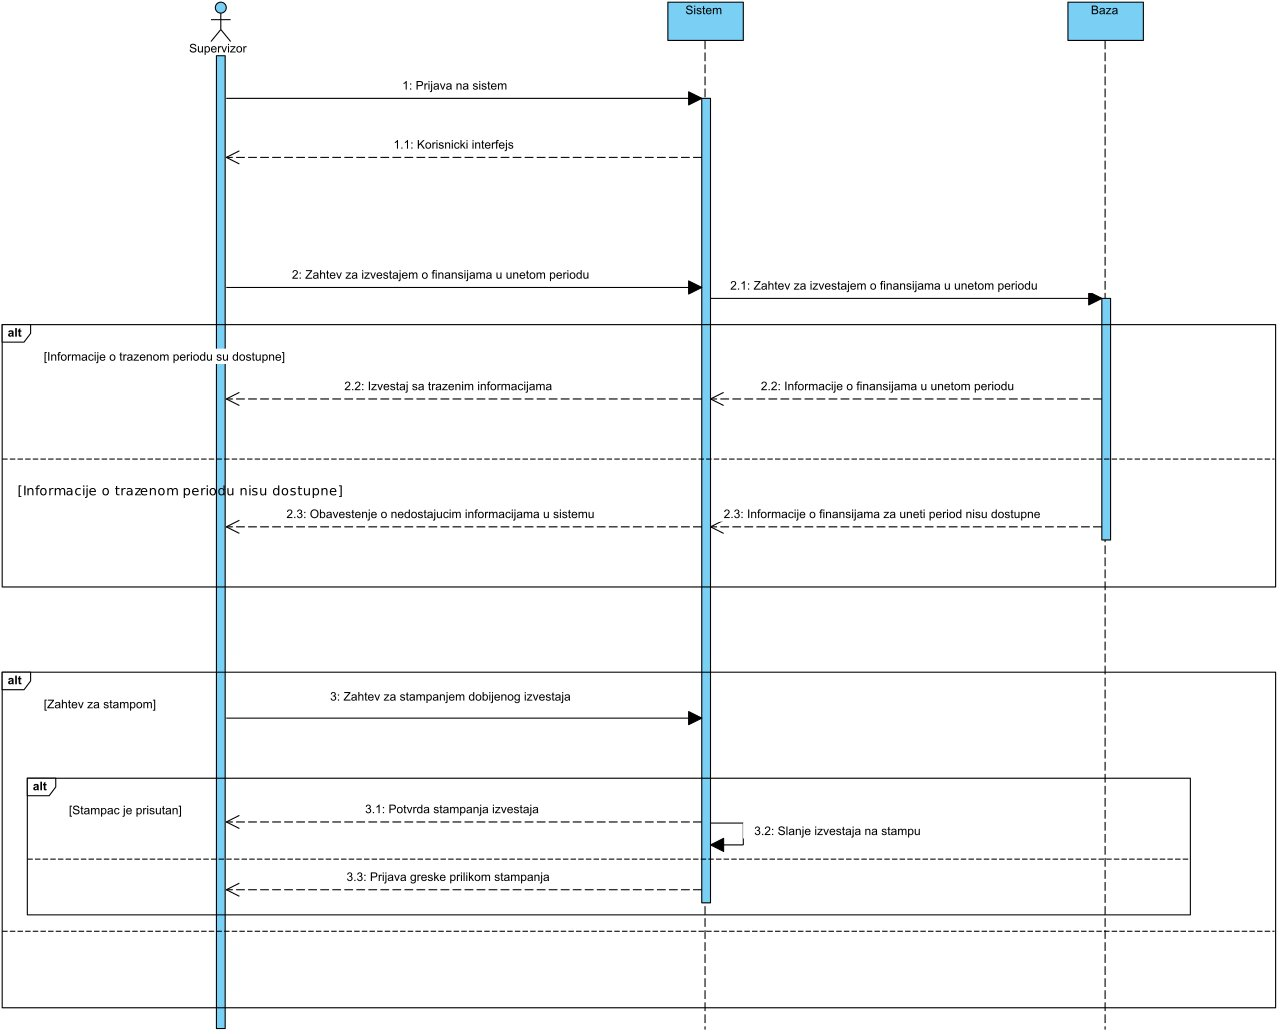
\includegraphics[width=100mm,height=100mm]{../images/sequence_vodjenje_finansija_1.jpg}
  \end{center}
  \caption{Dijagram sekvenci - Pregled finansija u vremenskom periodu}
  \label{sekvence_vodjenje_finansija_vreme}
\end{figure}


\subsubsection{Pregled finansija za konkretnu predstavu}
\noindent\textbf{Kratak opis:} Supervizor pozorišta može zatražiti pregled finansija vezanih za održavanje konkretne predstave

\noindent\textbf{Učesnici:} 
\begin{itemize}
  \item Supervizor pozorišta
\end{itemize}

\noindent\textbf{Preduslovi:} 
\begin{itemize}
  \item Supervizor pozorišta je prijavljen na sistem
\end{itemize}

\noindent\textbf{Postuslovi:} 
\begin{itemize}
  \item Supervizor je obavešten o svim finansijskim informacijama u vezi satrazenom predstavom
\end{itemize}

\noindent\textbf{Osnovni tok:} 
\begin{legal}
  \item Supervizor u sistemu otvara stranu za pregled finansija
  \item Supervizor unosi ime predstave za koju želi da sazna pregled finansija
  \item Sistem prikazuje podatke o finansijama za unetu predstavu
  \item Supervizor bira da li štampa izveštaj
\end{legal}

\noindent\textbf{Alternativni tokovi:}
\begin{itemize}
  \item \textbf{A1. Uneta predstava ne postoji u sistemu (korak 2)} 
      \begin{legal}
        \item Sistem obaveštava supervizora o problemu
        \item Proces se nastavlja u \textbf{koraku 1}.
      \end{legal}

  \item \textbf{A2. Štampač nije dostupan (korak 4)} 
  \begin{legal}
    \item Sistem obaveštava supervizora o problemu
    \item Proces se završava
  \end{legal}

\end{itemize}

\begin{figure}[H]
  \begin{center}
    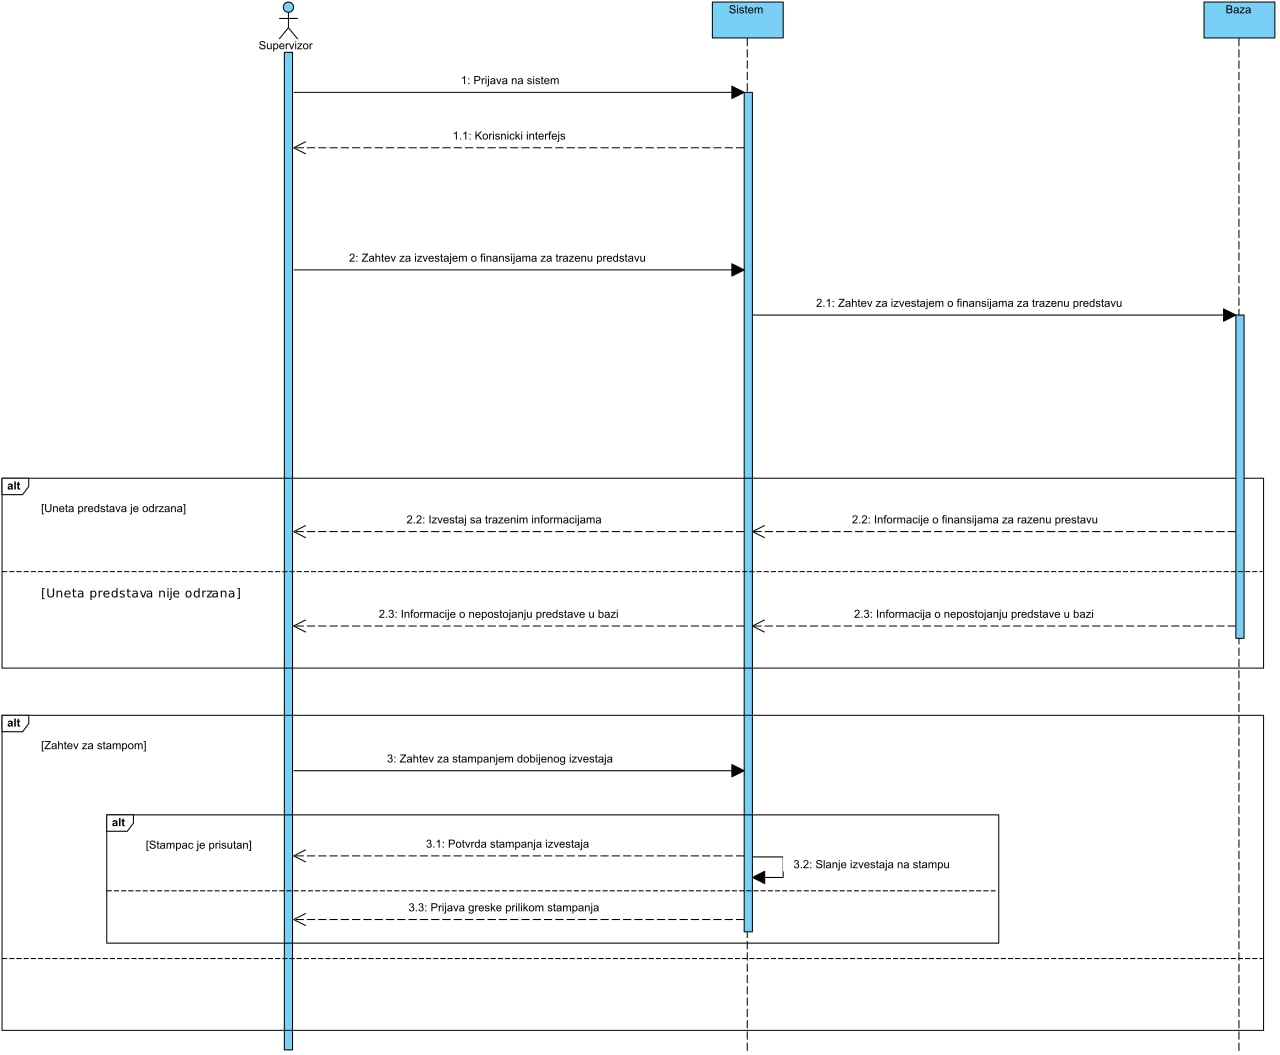
\includegraphics[width=100mm,height=100mm]{../images/sequence_vodjenje_finansija_2.jpg}
  \end{center}
  \caption{Dijagram sekvenci - Pregled finansija za konkretnu predstavu}
  \label{sekvence_vodjenje_finansija_predstava}
\end{figure}

\section{Druga sekcija.}
Ovo je druga sekcija.

\section{Treća sekcija.}
Ovo je treća sekcija.

\section{Zaključak}
Ovo je zaključak.

\newpage

\addcontentsline{toc}{section}{Literatura}
\appendix
\bibliography{literatura} 
\bibliographystyle{unsrt}

\end{document}
        
